\section{Teori}

För att beskriva fysikaliska fenomen används olika matematiska modeller. I våra simuleringar av vädrets inverkan på fastighetens energiflöden använder vi flera olika beräkningsmetoder. I det här avsnittet presenterar vi härledningar av de fysikaliska fenomen och beräkningsmetoder projektet använder sig av. Vi går också igenom definitioner av, för projektet, centrala begrepp.


\subsection{Värmeledning}
Konduktion. Det pågår ständigt värmetransport från kalla till varma sidor. Värmetransporten är proportionell mot temperaturskillnaden över konstruktionen. Konduktion, eller ledning genom ett material, här värmeledning innebär att värme flyttar sig inom ett material, utan att materialet i sig rör sig eller flyttar sig. Konduktiviteten, eller värmeledningsförmågan, betecknad kappa inom fysiken eller lambda inom byggsektorn är en materialegenskap. Eftersom överföring av värme i form av ledning är den enklaste överföringen är det den som lambda värdet bygger på. För att bestämma lambdavärdet för ett material utsätter man det för en temperaturskillnad och mäter den värmemängd som passerar genom materialet per tidsenhet. Då värmeöverföring via konvektion samt strålning är så pass svår att behandla matematiskt så ingår dessa i lambdavärdet som är väldigt enkelt att jobba med matematiskt. $q=k \nabla \cdot T$ vilket ger oss $Q=U \delta \cdot T$ och därifrån kan vi lösa ut U-värdet som $U = frac{Q}{\delta\ cdot T}$. Värmeledningsförmågan påverkas av materialets densitet, porositet, temperatur samt fuktighet. Fuktkorrigering görs, enligt vissa framställda värden. Värmemotstånd, R beräknas utifrån lambdavärdet.

\begin{equation}
Ri=\frac{d}{lambda}
\end{equation}

Överföringsmotstånd. Man påför sedan Rsi samt Rse, utsida samt insida. Beror på både strålnings samt konvektion. U-värdet beräknas som inversen av R-värdet. Har man olika material handlar det om att summera ihop 1/r.

\section{Svartkroppsstrålning}
\label{sec:blackbody}



Alla objekt reflekterar, absorberar och transmitterar ljus. De kroppar som varken reflekterar eller transmitterar något ljus utan absorberar 100\% kallas konventionellt för svartkroppar. Detta är en teorektisk konstruktion då perfekta svartkroppar inte existerar men trots detta kan en sådan användas som en god modell i flera fysikaliska tillämpningar. Den energi som absorberats strålas ut i form av svartkroppsstråling vars frekvensspektum bestäms av kroppens temperatur när kroppen är i termisk jämvikt med sin omgivning. Den totala utstrålade energin per tidsenhet fås ur Stefan-Boltzmanns lag


\begin{equation}\boxed{ \; \; \;
j^{\star} = \sigma T^{4}
\; \; \; }
\end{equation}

\noindent
där $\sigma$ är Stefan-Boltzmanns konstant som mäts i $\unit{s^{-1}m^{-2}K^{-4}}$ och $T$ är kroppens temperatur vid termisk jämvikt.

\subsection{Härledning}
% av stefan-boltzmanns lag
% med hål i en låda
% kolla i termoboken
I en låda med fotoner kan den totala energin inne i lådan beskrivas som 
\begin{equation}
\frac{U}{V}=\frac{8\pi^5}{15}\frac{(kT)^4}{(hc)^3}
\end{equation}

vilket fås ur Plancks spektrum.\cite{schroeder00}

Sedan görs ett litet hål i lådan, så att några av fotonerna kan slippa ut. Sannolikhet att fotoner med kort respektive lång våglängd ska slippa ut är samma som fördelningen mellan dem inne i lådan, eftersom de har samma hastighet.

\begin{figure}[hpbt]
\centering
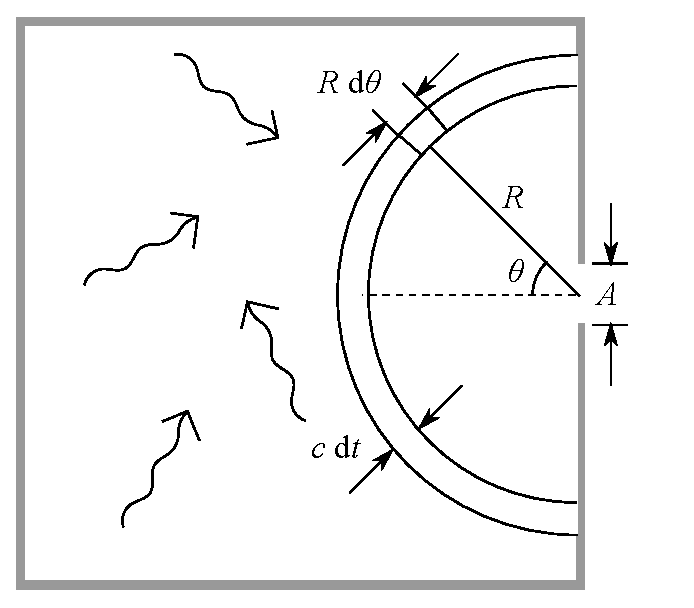
\includegraphics[height=0.3\textheight]{images/blackbody_box.eps}
\caption{\label{fig:box}{Fotonerna som lämnar lådan har en liten stund tidigare befunnit sig i samma hemisfär inne i lådan.}}
\end{figure}

Den totala mängden strålning som kommer ut kan då beräknas genom att tänka sig att de fotoner som når fram till hålet under en kort tidsperiod, $\mathrm{d}t$, alla befann sig i samma hemisfär inne i lådan för en liten stund sedan, se figur \ref{fig:box}. Tjockleken på den tänkta hemisfären är $c\mathrm{d}t$. Hemisfärens radie, $R$, beror givetvis på hur långt bak i tiden vi tittar.

Ett volymelement av hemsfären ges av
\begin{equation}
V=(R\mathrm{d}\theta) \times (R\sin\theta\mathrm{d}\phi) \times (c \mathrm{d}t).
\end{equation}

Energitäthetenför fotonerna i volymelementet är således
\begin{equation}
E_\text{v.e.}=\frac{U}{V} c \mathrm{d}t R^2 \sin\theta \mathrm{d}\theta \mathrm{d}\phi.
\end{equation}

Men endast den andel av fotonerna som har rätt riktning kommer ut genom lådans öppning. Sannoliketen för att en foton har rätt riktning är
\begin{equation}
P(\text{rätt riktning})=\frac{A\cos\theta}{4\pi R^2}
\end{equation}

där A är hålets area. Den totala energin som strålar ut ur hålet från det lilla volymselementet är alltså 
\begin{equation}
\frac{A\cos\theta}{4\pi}\frac{U}{V} c\mathrm{d}t \sin\theta\mathrm{d}\theta \mathrm{d}\phi
\end{equation}

vilket ger en total energiutstrålning på
\begin{equation}
\frac{A}{4}\frac{U}{V}c \mathrm{d}t
\end{equation}


\subsection{Konvektion}
\label{section:convection}
I fasta ämnen går det utmärkt att approximera värmeflöde enbart med hjälp
av värmeledningsekvationen. Detta håller dock ej lika bra för fluider, det vill säga
material som deformeras då de utsätts för tryck.
Under dessa förhållanden
måste det tas hänsyn till konservation av massa, energi samt rörelsemoment.
För att härleda giltiga differentialekvationer som beskriver en fluids rörelse används ofta sambandet

\begin{equation}
\label{eq:convection:reynolds}
\frac{dB}{dt} = \frac{d}{dt}\left( \int_{V} \frac{dB}{dm} \rho dV \right) + \int_{\partial V} \frac{dB}{dm} \rho \left( \mathbf{v} \cdot \mathbf{n} \right)dA,
\end{equation}

där $B$ är en godtycklig egenskap av fluiden, exempelvis dess rörelsemängd, V är den så kallade kontrollvolymen (omfattande ett godtyckligt valt område), $\partial V$ är denna kontrollvolyms rand, $\rho$ är fluidens densitet, $\mathbf{v}$ är fluidens hastighetsvektor och $\mathbf{n}$ är normalvektorn till randen. Detta samband benämns vanligen Reynolds transportteorem\footnote{För närmare beskrivning och härledning, se White, 2011 \cite{white11}}.

Sätt $B = m$ där $m$ är fluidens massa (oberoende av tiden) och låt $V$ vara en tidsoberoende volym. Ett uttryck för masskonservering erhålls:

\begin{equation}
\label{eq:convection:masscon}
\int_V \frac{\partial \rho}{\partial t} dV + \int_{\partial V} \rho \left( \mathbf{v} \cdot \mathbf{n} \right) dA = 0
\end{equation}

Första termen i detta uttryck beskriver förändringar i densiteten inom kontrollvolymen medan andra termen omfattar alla flöden in och ut genom kontrollvolymens rand. För masskonservering krävs alltså att summan av dessa termer ska vara noll. Den andra termen kan, vid diskreta flödesmängder, även skrivas som

\begin{equation}
\label{eq:convection:discrete}
\int_{\partial V} \rho \left( \mathbf{v} \cdot \mathbf{n} \right) dA = \sum_i \left( \rho \mathbf{v}_i\cdot \mathbf{A}_i \right)_{ut} - \sum_i \left( \rho \mathbf{v}_i\cdot \mathbf{A}_i \right)_{in}
\end{equation}

\begin{figure}[hpbt]
\centering
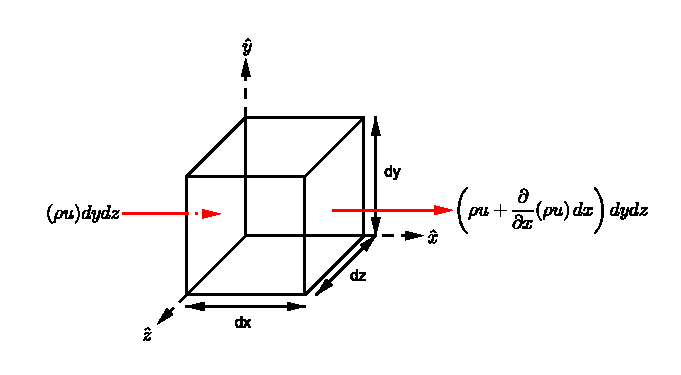
\includegraphics[scale=1]{images/massflowcube.eps}
\caption{\label{fig:massflowcube} Infinitesimal kontrollvolym för derivering av bevaranderelationer, här med massflödet exemplifierat}
\end{figure}

Betrakta nu en infinitesimal kontrollvolym som den i figur \ref{fig:massflowcube}. In- och utflödena kan här approximeras till endimensionella flöden och \eqref{eq:convection:masscon} reduceras till

\begin{equation}
\label{eq:convection:massconinf}
\int_V \frac{\partial \rho}{\partial t} dxdydz + \frac{\partial}{\partial x}\left( \rho u \right)dxdydz + \frac{\partial}{\partial y}\left( \rho v \right)dxdydz + \frac{\partial}{\partial z}\left( \rho w \right)dxdydz = 0
\end{equation}

vilket, om dxdydz tas bort, kan förenklas som

\begin{equation}
\label{eq:convection:continuity}
\frac{\partial \rho}{\partial t} + \nabla \cdot \left( \rho \mathbf{v} \right) = 0
\end{equation}

Om inkompressibilitet antas ($\rho$ = konstant) reduceras denna ekvation ytterligare till

\begin{equation}
\label{eq:convection:continuityinc}
\nabla \cdot \mathbf{v} = 0
\end{equation}

Detta är kontinuitetsekvationen för inkompressibla fluider.

Betrakta åter \eqref{eq:convection:reynolds} och sätt nu $B = m\mathbf{v}$. På samma vis som kontinuitetsekvationen \eqref{eq:convection:continuityinc} härleddes, fås för det infinitesimala volymelementet i figur sambandet

\begin{eqnarray}
\label{eq:convection:linear}
\sum \mathbf{F} & = & \frac{\partial}{\partial t} \left( \int_V \mathbf{v} \rho dV \right) + \sum_i \left( \dot{m}_i \mathbf{v}_i \right)_{ut} - \sum_i \left( \dot{m}_i \mathbf{v}_i \right)_{in}\nonumber\\
& = &\left(\frac{\partial}{\partial t} \left( \rho\mathbf{v} \right) + \frac{\partial}{\partial x}\left( \rho u \mathbf{v}\right) + \frac{\partial}{\partial y}\left( \rho v \mathbf{v}\right) + \frac{\partial}{\partial z}\left( \rho w \mathbf{v}\right)\right)dxdydz
\end{eqnarray}

ty enligt Newtons andra lag är tidsderivatan av rörelsemängden $m\mathbf{v}$ lika med summan av alla krafter som verkar på kroppen. $\dot{m}_i$ betecknar här massflödet $\rho\mathbf{v}_i\cdot\mathbf{A}_i$.

Det sista högerledet kan skrivas om som

\begin{equation}
\left( \mathbf{v}\left[ \frac{\partial \rho}{\partial t} + \nabla\cdot \rho \mathbf{v}\right] + \rho\left[ \frac{\partial \mathbf{v}}{\partial t} + u\frac{\partial\mathbf{v}}{\partial x} + v\frac{\partial\mathbf{v}}{\partial y} + w\frac{\partial\mathbf{v}}{\partial z} \right]\right)dxdydz.
\end{equation}

Första termen inom hakparentes är kontinuitetsekvationen \eqref{eq:convection:continuity} och går alltså bort. Den andra hakparentesen motsvarar något som kallas materiederivata. Man kan visa att 

% OBS, blandat tensorer och vektorer!
\begin{equation}
\label{eq:convection:material}
\frac{d\mathbf{v}}{dt} = \frac{\partial \mathbf{v}}{\partial t} + \mathbf{v}_i\frac{\partial \mathbf{v}}{\partial x_i}
\end{equation}

och därmed reduceras \eqref{eq:convection:linear} till

\begin{equation}
\label{eq:convection:linearfinal}
\sum \mathbf{F} = \rho \frac{d\mathbf{v}}{dt}dxdydz.
\end{equation}

Summan av de på volymen verkande krafterna måste nu utvecklas. Dessa krafter uppstår på grund av gravitation, tryck och viskositet. Andra krafter, såsom från elektromagnetiska fält, kan i sammanhanget anses vara försumbara. Gravitationskraften $\mathbf{F}_g$ beskrivs för den infinitesimala volymen med $\rho \mathbf{g} dxdydz = \rho g dxdydz \hat{z}$. Tryckkraften $\mathbf{F}_p$, i sin tur, ges av $-\nabla p dxdydz$. Viskositetskraften $\mathbf{F}_{visc}$ är lite besvärligare att sammanställa. Anta att volymen är en Newtonsk fluid, det vill säga stresstensorn $\tau$ är linjärt proportionell mot hastighetsgradienten $\nabla\mathbf{v}$ med proportionaltitetskonstanten $\mu$, $\tau = \mu \nabla \mathbf{v}$. 

% Hur härleda viskositetsbidraget

Vi har alltså ekvationssystemet

\begin{eqnarray}
\frac{du}{dt} & = & -\frac{\partial p}{\partial z} \nonumber\\
\frac{dv}{dt} & = & -\frac{\partial p}{\partial z}\\
\frac{dw}{dt} & = & \rho g -\frac{\partial p}{\partial z} \nonumber
\end{eqnarray}


För homogena inkompressibla fluider i två dimensioner gäller då ekvationerna
\eqref{eq:convection:continuity}, \eqref{eq:convection:momentumx},
\eqref{eq:convection:momentumz} samt \eqref{eq:convection:energy}. Här
är $\mathbf{v} = (u,w)$ hastighetsvektorn, $\alpha$ är den termiska
diffusiviteten, $\nu$ är den kinematiska viskositeten, $p$ är trycket,
$\rho$ är densiteten, $g$ är den lokala tyngdaccelerationen
och slutligen är $\rho_0$ referensdensiteten.

\begin{equation}
\label{eq:convection:momentumx}
\frac{\partial u}{\partial t} + \mathbf{v}\cdot\nabla u = 
-\frac{1}{\rho_0}\frac{\partial p}{\partial x} + 
\nu\Delta u
\end{equation}

\begin{equation}
\label{eq:convection:momentumz}
\frac{\partial w}{\partial t} + \mathbf{v}\cdot\nabla w = 
-\frac{1}{\rho_0}\frac{\partial p}{\partial z} + \nu\Delta w - \frac{\rho}{\rho_0}g
\end{equation}

\begin{equation}
\label{eq:convection:energy}
\frac{\partial T}{\partial t} + \mathbf{v}\cdot\nabla T = \alpha\Delta T
\end{equation}

\subsubsection{Boussinesq approximation}

För flytkraftsdrivet flöde kan det vara lämpligt att använda sig av
Boussinesq approximation. Denna säger att det enda som påverkar trycket är
tyngdaccelerationen. Genom detta är det möjligt att sätta upp uttryck för densiteten
och tryckderivatorna enligt ekvationerna \eqref{eq:convection:density}
och \eqref{eq:convection:pressurez}. Här är
$\beta$ den volymetriska expansionskonstanten och
$T_0$ temperaturen som råder vid referensdensiteten $\rho_0$.

\begin{equation}
\label{eq:convection:density}
\rho = \rho_0[1-\beta(T-T_0)]
\end{equation}

\begin{equation}
\label{eq:convection:pressurez}
\frac{\partial p}{\partial z} = -\rho_0g
\end{equation}



\subsection{Finita element av inkompressibel fluid}

För att lösa Navier-Stokes ekvationer kan lämpligen en datormodell användas.
Här består denna modell av ett system uppsatt med Galerkins metod.
I denna lösning så begränsar vi dock oss till att enbart behandla statiska flöden
vilket genomförs genom att sätta alla tidsderivator till noll.

För att hantera trycket i \eqref{eq:convection:continuity}-\eqref{eq:convection:energy} används den tidigare nämnda Boussinesq approximation
samt penalty metoden för att göra hastighetsvektorn källfri och uppfylla
kontinuitetsekvationen. Det finns således inget direkt behov av att räkna ut trycket.
Vid användning av många sorters elementtyper som inte uppfyller Babuska-Brezzikriteriet
är detta dessutom nödvändigt då det annars kan bildas oönskade trycknoder. 
En annan möjlighet är att välja divergensfria element. \cite{babuska1973}\cite{segal2011}

Genom penaltymetoden beskrives här trycket som $p$ enligt ekvation
\eqref{eq:femconvection:penalty}. Här är $p_s$ någon form av idealt statiskt
tryck som är önskat. Detta tryck följer Boussinesq approximation. Med dessa
idealiseringar kan differentialekvationerna sättas upp igen. \cite{heinrich88}\cite{taylor79}
Som kan ses så leder den godtyckliga penaltyparametern $\lambda$ till att justera trycket
om hastighetsfältets divergens ej är identiskt noll. I viss litteratur anges 
det att penaltyparametern skall vara i storleksordningen $10^7$ men att den
är väldigt applikationsberoende. En för liten vald penaltyparameter leder till att
trycket inte elimineras. Andra problem uppstår vid en för stor parameter. Ekvationssystemet
kan bli svårlöst och få stabilitetsproblem när parametern blir
för stor i jämförelse med de andra delarna i differentialekvationen.\cite{reddy93}\cite{roy05}\cite{basak04}\cite{segal2011}

\begin{equation}
\label{eq:femconvection:penalty}
p = p_s - \lambda\nabla\cdot\mathbf{v}
\end{equation}

\noindent
Fortsatt skall trycket deriveras med avseende på de rumsliga variablerna vilket möjliggör
att eliminera trycket från differentialekvationerna. Dessa deriveringar kan ses i ekvation
\eqref{eq:femconvection:partx} samt \eqref{eq:femconvection:partz}. Notera att det statiska trycket
$p_s$ ej beror på $x$ vilket resulterar i att derivatan är noll.

\begin{equation}
\label{eq:femconvection:partx}
\frac{\partial p}{\partial x} = \frac{\partial p_s}{\partial x} -
\frac{\partial}{\partial x} \lambda\nabla\cdot\mathbf{v} = -
\frac{\partial}{\partial x} \lambda\nabla\cdot\mathbf{v}
\end{equation}

\begin{equation}
\label{eq:femconvection:partz}
\frac{\partial p}{\partial z} = \frac{\partial p_s}{\partial z} -
\frac{\partial}{\partial z} \lambda\nabla\cdot\mathbf{v} =
-g\rho_0 - \frac{\partial}{\partial z} \lambda\nabla\cdot\mathbf{v}
\end{equation}

\noindent
Detta förs in i momentekvationerna vilket ger ekvationerna \eqref{eq:femconvection:u} -
\eqref{eq:femconvection:T}. Här är det ekvationssystem som syftar att lösas.

\begin{equation}
\label{eq:femconvection:u}
\mathbf{v}\cdot\nabla u =
\frac{\lambda}{\rho_0}\nabla\cdot\mathbf{v} +
\nu\Delta u
\end{equation}

\begin{equation}
\label{eq:femconvection:w}
\mathbf{v}\cdot\nabla w =
\frac{\lambda}{\rho_0}\nabla\cdot\mathbf{v} + \nu\Delta w +g\beta(T-T_0)
\end{equation}

\begin{equation}
\label{eq:femconvection:T}
\mathbf{v}\cdot\nabla T = \alpha\Delta T
\end{equation}

\subsubsection{Svag formulering}

En finita elementlösning med Galerkins metod kräver att problemet reduceras till
ett ekvivalent variationsproblem. Här söks $T\in\Phi$, $u\in\Phi$ och
$w\in\Phi$ som uppfyller ekvation \eqref{eq:femconvection:variation}. Här
betecknar brackets skalärprodukt, $\mathbf{L}$ är differentialoperatorn
som betecknar systemet av differentialekvationer som $\mathbf{L}(T,u,w) = 0$.
$\Phi$ är rummet av alla testfunktioner $\phi$ som är kontinuerliga i
definitionsmängden $\Omega$ samt vars derivator är bitvis kontinuerliga på randen
$/Gamma$. De måste även vara $L^2$ integrabla.

\begin{equation*}
\label{eq:femconvection:variation}
\langle \mathbf{L}(T,u,w), \phi \rangle = 0\mbox{,  } \forall \phi \in \Phi
\end{equation*}


\section{Optimering med Newton-Raphsons metod}

När ett ekvationssystem är ickelinjärt kan ej exakta metoder som Gausseliminering användas
för ekvationslösning. Detta stötte vi till exempel på vid finita elementlösningen
av Navier-Stokes ekvationer i avsnitt \ref{sec:femconvection}.
I dessa fall måste approximativa optimeringsmetoder utnyttjas. En sådan
metod är Newton-Raphsons metod. Denna bygger på trunkerad Taylorutveckling 
av en funktion för att linjarisera ett ickelinjärt ekvationssystem
$\mathbf{f}(\mathbf{x}) = 0$
vilket kan ses i ekvation \eqref{eq:newtonsmethod:taylor}. Här är
$\mathbf{J}_f(\mathbf{x})$ jacobianen för $\mathbf{f}(\mathbf{x})$. 

\begin{equation}
\label{eq:newtonsmethod:taylor}
\mathbf{f}(\mathbf{x} + \Delta\mathbf{x}) \approx \mathbf{f}(\mathbf{x}) +
\mathbf{J}_f(\mathbf{x})\Delta\mathbf{x}
\end{equation}

\noindent
Principen går ut på att algoritmen upprepat gissar nya lösningar där de
nya lösningarna följer den negativa jacobianen. Till en början är en god initial gissning
$\mathbf{x}_0$ ett kriterie för att Newton-Raphson skall konvergera. Därefter så beräknas
funktionsvärdet $\mathbf{f}(\mathbf{x}_0)$ samt jacobianen $\mathbf{J}_f(\mathbf{x}_0)$.
Dessa används för att beräkna nästa gissning genom att lösa
\eqref{eq:newtonsmethod:guess} och beräkna nästa $\mathbf{x}$ med
\eqref{eq:newtonsmethod:nextx}. \cite{heath2002}

\begin{equation}
\label{eq:newtonsmethod:guess}
\mathbf{J}_f(\mathbf{x}_n)\Delta\mathbf{x}_n = -\mathbf{f}(\mathbf{x_n})
\end{equation}

\begin{equation}
\label{eq:newtonsmethod:nextx}
\mathbf{x}_{n+1} = \mathbf{x}_n + \Delta\mathbf{x}_n
\end{equation}

\noindent
Itereringen bör avbrytas då ett maxantal itereringar har uppnåtts och funktionen
ej har konvergerat alternativt när felet är tillräckligt litet. En av styrkorna 
med denna algoritm är dess kvadratiska konvergens mot enkelrötter. \cite{ympa95}
En svaghet med Newton-Raphson är att det i många fall ej är möjligt att analytiskt beräkna
jacobianen. Istället måste andra algoritmer untnyttjas som till exempel finita differensmetoden
för beräkning av jacobianen. Omvägar som denna bidrar till att lösningsprocessen blir mycket
mer omständig och processorintensiv. 

\subsection{Konvergens samt konvergenskriterier}

För att enklare förstå några problem som kan uppstå med Newton-Raphsons metod kan det vara lämpligt
att repetera beviset av dess kvadratiska konvergens. Definiera en funktion $f(x)$ enligt \eqref{eq:newtonproof}.
Antag att den roten $f(x) = 0$ existerar för $x = \alpha$.

\begin{align}
f: & \mathbb{R} \to \mathbb{R} \nonumber \\
   & x \mapsto f(x) \label{eq:newtonproof}
\end{align}

\noindent
Härnäst genomförs en taylorutveckling av funktionen $f(x)$ i ekvation \eqref{eq:newtonprooftaylor}.
Den kvadratiska termen är här Lagranges restterm med parametern $\xi_n \in [\alpha, x_n]$.

\begin{equation}
\label{eq:newtonprooftaylor}
f(\alpha) = f(x_n) + f^\prime(x_n)(x_n-\alpha) + \frac{f^{\prime\prime}(\xi_n)}{2}(x_n-\alpha)^2
\end{equation}

\noindent
Nu kan förstaderivatan av $f(x_n)$ divideras över samt $f(\alpha)$ är känt att vara noll.
Efter detta identifieras $f(x_n)/f^\prime(x_n) = x_n-x_{n+1}$ och ersätts. Slutligen så ses
det i ekvation \eqref{eq:newtonqed} att $x_{n+1}-\alpha \propto (x_{n}-\alpha)^2$.

\begin{equation}
0 = \frac{f(x_n)}{f^\prime(x_n)} + \alpha - x_n + \frac{f^{\prime\prime}(\xi_n)}{2f^\prime(x_n)}(x_n-\alpha)^2
\Rightarrow
\end{equation}

\begin{equation}
\label{eq:newtonqed}
x_{n-1} - \alpha = - \frac{f^{\prime\prime}(\xi_n)}{2f^\prime(x_n)}(x_n-\alpha)^2 
\end{equation}

\noindent
För att ovanstående bevis ska gälla så måste andraderivatan vara uppåt begränsad, förstaderivatan får ej
vara noll och den högre ordningens derivator får ej vara av stor betydelse för funktionens uppträdande
nära roten $f(x) = 0$. Rent praktiskt innebär detta att en god gissning är essentiell för att få
konvergens i metoden. Även med en god gissning så kan problem uppstå om derivatan av funktionen
förändras snabbt i omgivningen av $x$. Detta kan resultera i både att nästa gissning ligger för långt
bort och för nära. Det förstnämnda problemet innebär att metoden hoppar över roten vilket till och med
kan innebära att metoden divergerar. Det andra problemet är mindre allvarligt då det enbart innebär 
att metoden förlorar sin kvadratiska konvergens.

\subsection{Förbättrad Newton-Raphson}

En metod för att hantera att metoden hoppar över rötter är att i varje steg försöka minimera $|f(x_{n+1})|$.
Rent praktiskt innbär detta att vi väljer en konstant $0 \le k_n \le 1$ och genomför ett modifierat
Newtonsteg enligt ekvation \eqref{eq:newtonmodified}.

\begin{equation}
\label{eq:newtonmodified}
x_{n+1} = x_n - k_n\frac{f(x_n)}{f^\prime(x_n)}
\end{equation}

\noindent
För att identifiera det optimala valet av $k_n$ kan godtycklig linjesökningsalgoritm användas. Ett val av metod
är att behandla det analytiskt för att göra metoden mindre processorintensiv. En ny funktion definieras
enligt ekvation \eqref{eq:newtong} med $\Delta x_n = f(x_n)/f^\prime(x_n)$.

\begin{equation}
\label{eq:newtong}
g(k_n) = f(x_n- k_n\Delta x_n)
\end{equation}

\noindent
I ekvation \eqref{eq:newtongmin} deriveras funktionen med avseende på $k_n$ i punkten $k_n=0$
och kedjeregeln används för att skriva om uttrycket till något som är användbart.

\begin{align}
\frac{\partial g(k_n)}{\partial k_n}\,\bigg|_{k_n=0} & = 
\left(\frac{\partial g(k_n)}{\partial (k_n\Delta x_n)}
\frac{\partial k_n \Delta x_n}{\partial k_n}\right)\,\bigg|_{k_n=0} = \nonumber \\
x_n \frac{\partial f(x_n- k_n\Delta x_n)}{\partial (k_n\Delta x_n)}\,\bigg|_{k_n=0} & = 
-\Delta x_n f^\prime(x_n) = - f(x_n)
\label{eq:newtongmin}
\end{align}

\noindent
Ett förslag på algoritm är nu att i varje iterationssteg först beräkna det fulla newtonsteget motsvarande $k_n=1$.
Är då $f(x_{n+1}) < f(x_n)$ så kan steget godtagas. Stämmer inte detta så beräkas derivatan av $g(k_n)$ och
funktionen $g(k_n)$ ansätts vara ett polynom av andra ordningen enligt ekvation \eqref{eq:newtonfit}.

\begin{equation}
\label{eq:newtonfit}
g(k_n) = ak^2_n + bk_n + c
\end{equation}

\noindent
Nu kan de kända värdena $g(0)$, $g(1)$ samt $g^\prime(0)$ användas för att lösa ut koefficienterna i polynomet.
Dessa kan slutligen användas för att beräkna derivatan av $g(k_n)$ för att hitta dess minimum och således
hitta den optimala parametern $k_n$.

\noindent
Om denna metod skall användas för att lösa ett ekvationssystem istället för en realvärd funktion i en dimension
så behövs något mått sättas upp. Problemet som önskas att lösas är $\mathbf{F}(\mathbf{x}) = 0$.
Funktionen som skall minimeras kan då med fördel väljas till $f(\mathbf{x}) = \mathbf{F}(\mathbf{x})^2/2$.
På ett analogt sätt ovan så beräknas derivatan av funktionen $g(k)$ till ekvation \eqref{eq:newtonvecg}.\cite{fortran77}

\begin{equation}
\label{eq:newtonvecg}
g_n^\prime(0) = - \mathbf{F}(\mathbf{x_n})^2 \le 0
\end{equation}

\noindent
För att hitta roten $\mathbf{F}(\mathbf{x}) = 0$ så ansätts som ovan ett polynom där koefficienterna beräknas.
Som kan ses så existerar det ett $k_n$ så att $\mathbf{F}(\mathbf{x}_{n+1}) \le \mathbf{F}(\mathbf{x}_n)$ ty
$g^\prime(0) \le 0$ och enbart noll om roten redan är funnen.


\section{Kvantifiering av konstanta energiflöden}

Flera av energiflödena genom fastigheten är relativt konstanta sett till en längre tidsperiod. Det gäller främst värme från elektriska apparater, så som kylskåp och datorer, människors kroppsvärme och varmvattencirkulation. På så sätt kan aktivt tillförd energi, det vill säga den energitillförsel som kan regleras och tillförs via radiatorerna, enkelt regleras med hänsyn till dessa, om man bara känner dess storlek.

\subsection{Uppvärmning från människor}
Den utstrålade kroppsvärmen från människor kan beräknas genom att de antas vara svartkroppar. Stefan-Boltzmanns lag säger då att utstrålade energi per yt- och tidsenhet är $j=\sigma T^4$, där $T$ är temperaturen och $\sigma=\unit[5.6705\cdot 10^8]{Wm^{-2}K^{-4}}$ \cite{physicshandbook}, se teoriavsnitt \ref{sec:blackbody}. På samma sätt beräknas den energi som strålas in mot kroppen från omgivningen. Nettostrålningen från en människa kan då ses i ekvation \eqref{eq:constantsources:stefan} där $T_k=37^{\circ}C=310K$ är kroppstemperaturen och $T_r=20^{\circ}C=293K$ är rumstemperaturen. Multipliceras det med en människas area, ungefär $\unit[2]{m^2}$, fås en nettoeffekt på $\unit[211]{W}$. I själva verket reduceras denna effekt av en rad faktorer. Exempelvis är hudens temperatur lägre än kroppstemperaturen samtidigt som klädesplagg reducerar effektutstrålningen något. Professor Göran Grimvall skriver i NyTeknik att en rimlig nettoeffekt vid vila är cirka 1 W per kilogram kroppsvikt, alltså ungefär $\unit[50-100]{W}$\cite{Grimvall}.

\begin{equation}
\label{eq:constantsources:stefan}
j=\sigma \left( T_k^4 - T_r^4 \right)
\end{equation}
\noindent

\subsection{Varmvattencirkulation i fastigheten}
I huset cirkulerar hela tiden varmvattnet för att alltid kunna tillgodose de boendes behov av varmvatten utan dröjsmål. Efter en tur i systemet sjunker temperaturen på varmvattnet med tre grader och flödet är $\unit[800]{l/h}$. Detta motsvarar en energitillförsel till fastigheten på $\unit[2,8]{kW}$.

\subsection{Energi från elektrisk apparatur}
Den största delen av energin som driver en elektrisk apparat blir till värme. Därför låter vi energiflödet från elektriska apparatur motsvaras av fastighetens energiförbrukning, vilken kan läsas av kontinuerligt och på så sätt bli en del av reglersystemet.


\section{Effektflöde genom fönster på grund av solstrålning}

Solstrålning genom fönster orsakar snabba temperaturökningar i inomhusklimatet. Hur snabba och stora dessa temperaturökningar blir beror på en mängd parametrar varav de viktigaste omfattas av fönstrets utformning, det vill säga glasets reflektivitet och emmissitivitet, strålningens infallsvinkel som beror av tid på dagen och året och ytorna inomhus som solstrålningen faller på, så som persienner, gardiner, vägger och möbler. Fönstrets reflexivitet och emmisivitet är beror av solens infallsvinkel.

%\begin{itemize}
%\item{
%fönstrets utformning, det vill säga glasets reflektivitet och emmissitivitet.
%}
%\item{
%vinkeln relativt fönstret som strålningen infaller vid, det vill säga tid på dagen och året. Detta är starkt förknippat med föregående punkt. 
%}
%\item{
%de inomhus belägna ytorna som solstrålningen faller på, det vill säga persienner, gardiner, väggar, möbler, etcetera.
%}
%\end{itemize} 

\subsection{g-värden}\label{gvalue}

För att ange transmittansen av solstrålning genom fönster brukar man använda vad som kallas för g-värden (ibland även kallat ''Solar Factor''). Detta värde, mellan noll och ett, anger hur mycket av vinkelrätt infallande solstrålning som släpps igenom. Men eftersom ett sådant värde också beror på strålningens infallsvinkel är den ofta svår att beräkna.
% hur kan det både bero och inte bero av vinkeln?

Enligt \cite{karlssonroos99} förändras detta vinkelberoende främst med antalet glas (flerglasfönster) samt typ av eventuella beläggningar på glaset. I samma artikel visades också att g-värdenas vinkelberoende kan approximeras med ett polynom

\begin{equation}\label{eq:radiationwindowstheory:gvalue}
g = g_0 \left( 1 - az^{\alpha} - bz^{\beta} - cz^{\gamma} \right)
\end{equation}

där $g_0$ är g-värdet då strålningen infaller vinkelrätt mot ytan, $a+b+c=1$ och $z=\theta/90$ då $\theta$ är vinkeln, mätt i grader, mellan fönstrets normal och solstrålningens riktning. Koefficienterna och exponenterna i \eqref{eq:radiationwindowstheory:gvalue} beror på typen av fönster, och kan sättas till
% Varför kan man sätta dem till det här? vad betyder det?

\begin{align}\label{eq:gconstants}
a & = 8, & b & = 0.25/q, & c & = (1-a-b) \nonumber \\
\alpha & = 5.2 + 0.7q, & \beta & = 2, & \gamma & = (5.26+0.06p) + (0.73+0.04p)q
\end{align}

där p är antalet rutor i fönstret (treglasfönster medför $p = 3$) och q är en parameter, $1 \le q \le 10$, som varierar beroende på beläggningar på glasets yta. Exempelvis har ett treglasfönster utan beläggningar värdet $q=4$.

Det beräknade g-värdet kan sedan användas för att uppskatta energiflödet genom fönstret. Anta att en pyranometer anger solstrålningsintensiteten $I_0$ i $\unit{W m^{-2}}$. Då ges det totala energiflödet Q av sambandet $Q = g \cdot A \cdot I_0 \cos{\theta}$ i $\unit{W}$, där $A$ är fönstrets area och $\theta$ är vinkeln solen bildar mot ytans normal.

\section{En beskrivning av fastigheten på Walleniusgatan och dess konstruktion}
\label{subsec:thehouse}
% Johanneberg 7:8

% Hur tänkte de när de byggde och renoverade huset?
% Vad ville de uppnå och vilka regler och normer hade man att hålla sig till?

% Att huset är byggt så här vad betyder det för hur huset påverkas och hur huset är att bo i?

% Det är så här stort och har så här många rum, så här högt i tak o.s.v. 

Huset uppfördes 1935\cite{ritningar_urspr} och sedan kom det att dröja ända till 1988 innan den första större ombyggnationen gjordes. Då gjordes två lägenheter om till kontor, stammar byttes och vinden byggdes om till lägenheter. Både taket, burspråken på södersidan och den norra fasaden tilläggsisolerades. I samband med detta installerades också nya värme- och ventialtionssystem och alla fönster tätades med expanderskum. Den främsta skillnaden för de boende blev minskat drag och bättre luftgenomströmmning.  Med det nya venitlationssystemet byts luften helt och hållet varannan timme. Enligt Peter Särneö\cite{petersarneo} förbrukar fastigheten idag mindre energi än ett nybyggt hus.

Fastigheten 13 lägenheter och en kontorslokal på $\unit[225]{m^2}$. De utgör tillsammans $\unit[1450]{m^2}$ fördelat på sju våningar. Utöver detta finns det gemensamma utrymme, trapphus, förråd och apparatrum i den nedre källaren och Peter Särneö\cite{petersarneo} bedömmer att det totalt rör sig om ca $\unit[2000]{m^2}$. Sedan ett tag tillbaka har även en väderstation installerats i förhoppningen att den ska kunna utnyttjas för att förbättra fastighetens klimat ytterligare, se avsnitt \ref{subsec_weathertransmitter}.


% De olika gränsytornas material och uppbyggnad.
\subsection{Väggarna}

Ytterväggarna bestod ursprungligen av 50 cm tegel, klätt med ett centimetertjockt lager av puts på insidan, se figur \ref{fig:sodervagg}. Norrväggen, som tilläggsisolerades i samband med renoveringen 1988, har dessutom 2 cm puts, 10 cm mineralull och ytterligare 2 cm puts utanpå tegelväggen, se figur \ref{fig:norrvagg}.\cite{kandidatarbete2010}\cite{petersarneo}

\begin{figure}[hpbt]
\centering
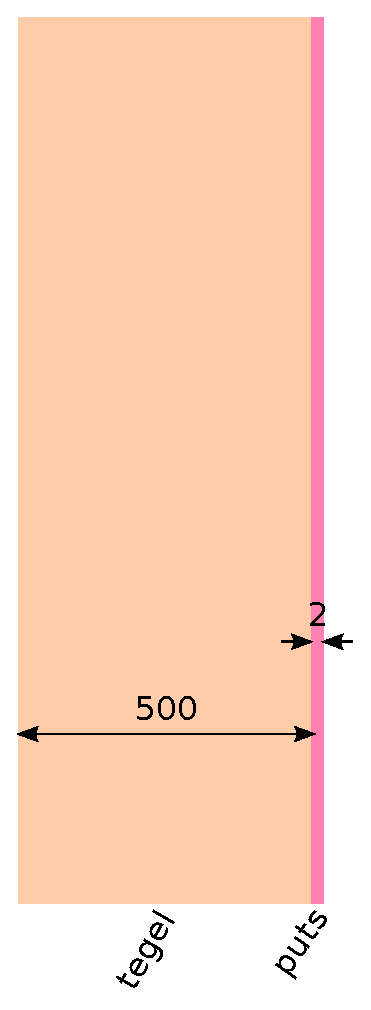
\includegraphics[height=0.3\textheight]{images/sodervagg.eps}
\caption{\label{fig:sodervagg}{Söderväggen, utifrån och in från vänster till höger. Alla mått är i mm.}}
\end{figure}

\begin{figure}[hpbt]
\centering
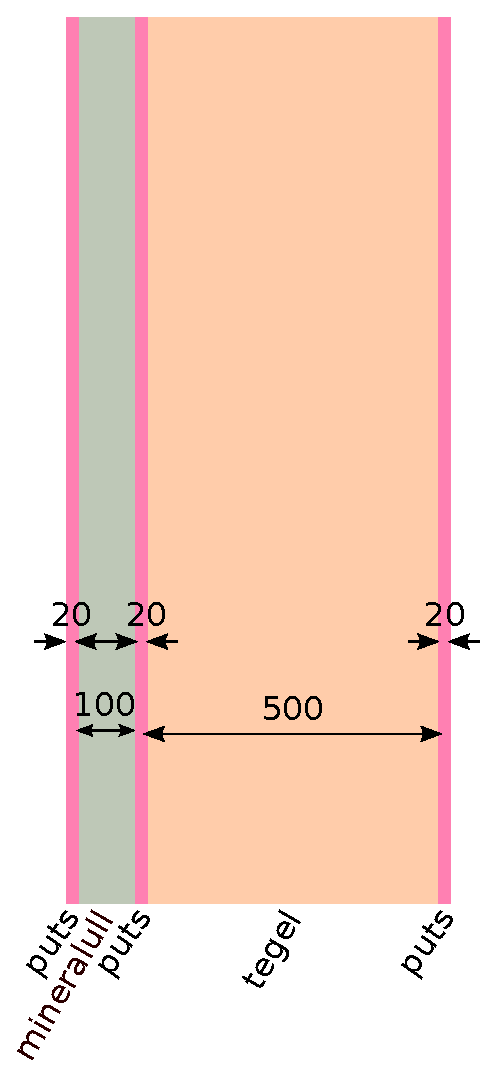
\includegraphics[height=0.3\textheight]{images/norrvagg.eps}
\caption{\label{fig:norrvagg}{Norrväggen, utifrån och in från vänster till höger. Alla mått är i mm.}}
\end{figure}

Fastigheten mellan två andra byggnader i liknande stil. Det öster om är lika högt som fastigheten medan det i väster är något lägre. Fastighetens yttervägg i väster är inte tilläggsisolerad och har samma uppbyggnad som söderväggen, se figur \ref{fig:sodervagg}.

På söderväggen finns ett burspråk som är kopparklätt kopparn sitter direkt på en cementbunden spånskiva och sedan en luftspalt om ca 2,5 cm. Väggen innanför består av 1,6 cm gips, 5 cm minneralull och sedan ytterligare 2,4 cm gips, se figur \ref{fig:bursprak}.\cite{kandidatarbete2010} Enligt Peter Särneö\cite{petersarneo} är det burspråket som läcker mest energi.

\begin{figure}[hpbt]
\centering
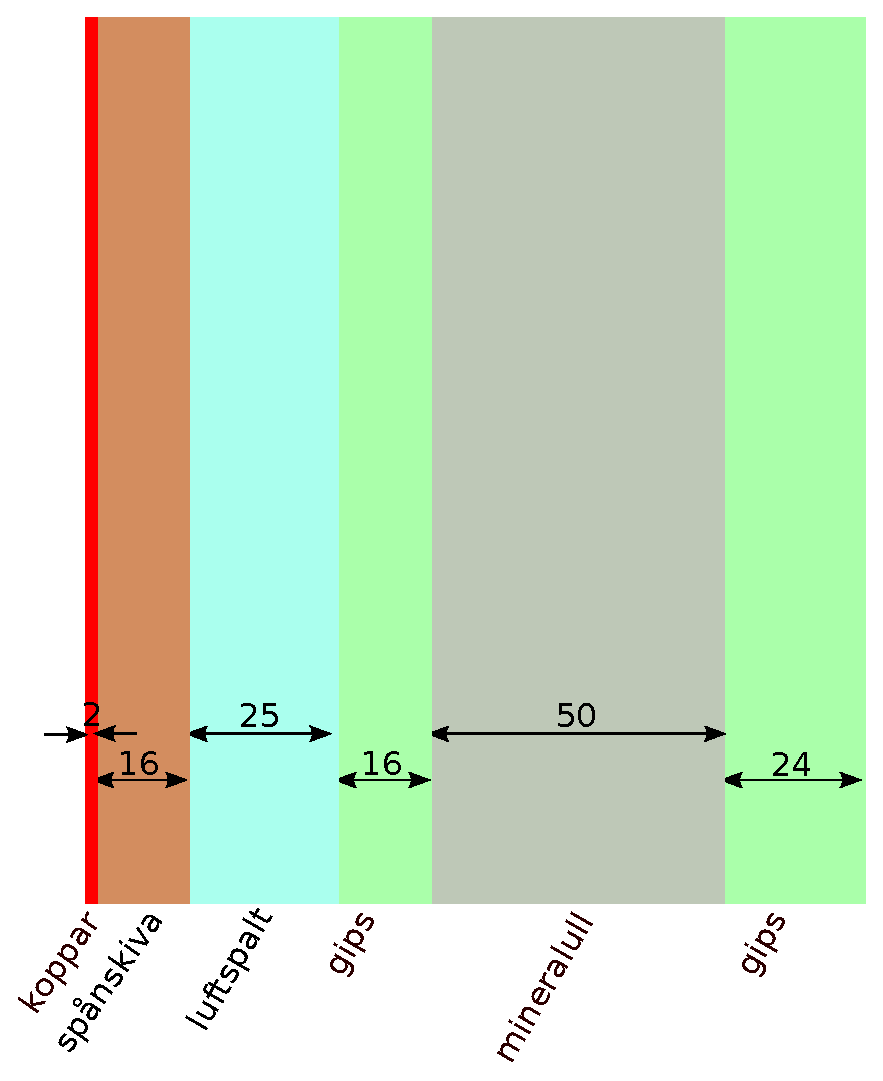
\includegraphics[width=0.3\textheight]{images/bursprak.eps}
\caption{\label{fig:bursprak}{Burspråket på söderväggen, utifrån och in från vänster till höger. Alla mått är i mm.}}
\end{figure}

\subsection{Taket}
Även taket lades om i samband med den stora renoveringen för minskad energiåtgång. Efter det bestod det av taktegel på underlagspapp ytterst, följt av 1,3 cm gips, 21 cm mineralull och innerst ytterligare 2,6 cm gips, se figur \ref{fig:taket}.\cite{kandidatarbete2010}

\begin{figure}[hpbt]
\centering
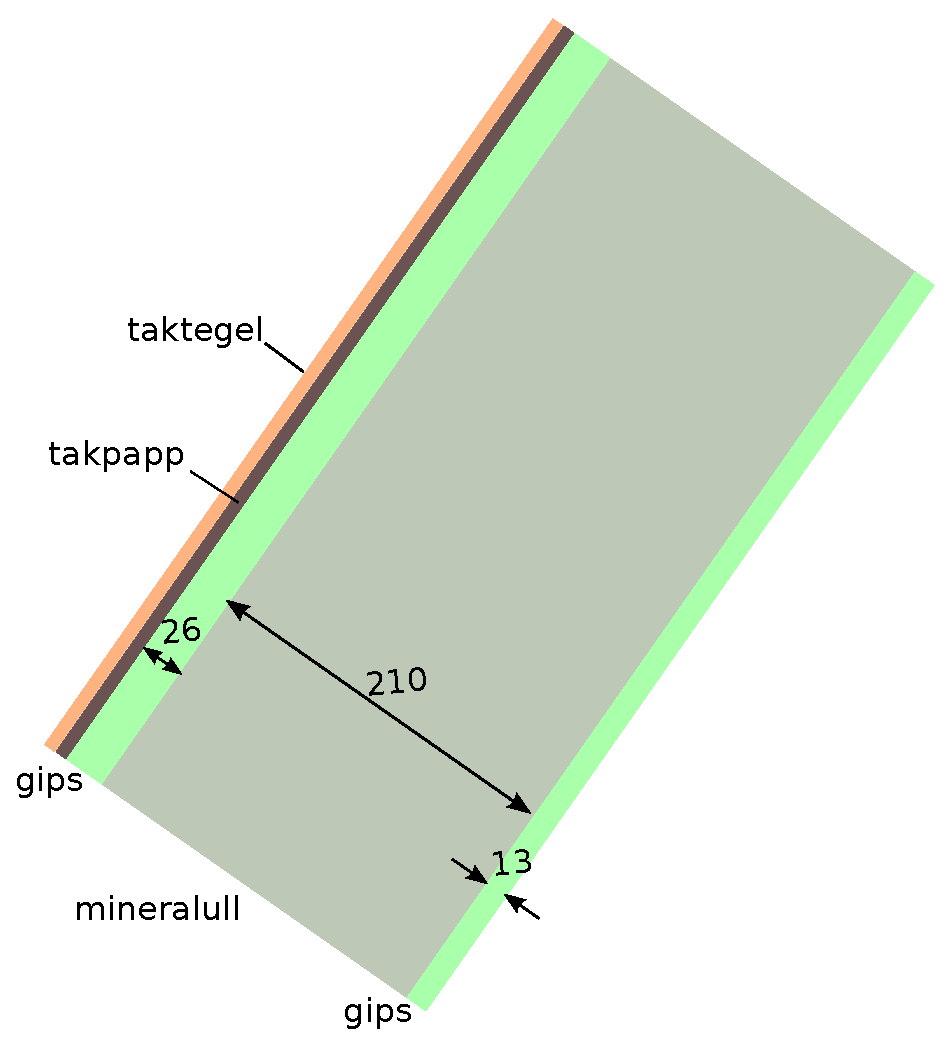
\includegraphics[width=0.3\textheight]{images/taket.eps}
\caption{\label{fig:taket}{Takets uppbyggnad. Alla mått är i mm.}}
\end{figure}

\subsection{Fönstren}

Byggnadens fönster är av treglastyp utan ytbeläggningar. Utrymmet mellan de två innersta glasskivorna är fyllt med argon för att minska värmeledningsförmågan. Totalt får fönstren ett U-värde på ungefär $\unit[1]{W/m^2}$, se avsnitt \ref{sec:heatconduction}. 

\subsection{Grunden}

Huset är byggt på ett berg som sluttar kraftigt. I östra delen av fastigheten ligger huset direkt på berget med endast ett lager av makadam emellan\cite{petersarneo}. I västra halvan har huset en undre källare, det är där apparat- och fläktrummen finns. Där är det betydligt större avstånd ned till berget, uppskattningsvis ett par meter. % Mer exakt? Källa?

\subsection{Uppvärmning och ventilation}
Idag värms huset av bergvärme från tre bergvärmepumpar. För att minska energiåtgången har ett flertal värmeväxlare installerats och värmen från all frånluft återanvänds i möjligaste mån.
% Hur fungerar regleringen? Källa?
Det är viktigt att lägenheterna är kalibrerade så att de får samma temperatur vid samma energiutflöde.

\section{Definition av väder för tillämpningar i denna rapport}
\label{subsec_weather}
Vår uppdragsgivare vill undersöka hur inomhustemperaturen påverkas av vädret. Tesen är att man kan få en mer korrekt styrning av inomhustemperaturen om man inte bara låter den påverkas av utomhustemperaturen, utan även av fler väderparamterar. Han har därför installerat en väderstation, se avnitt~ \ref{subsec_weathertransmitter}.
Begreppet väders vardagliga användningsområde är mycket brett och behöver därför avgränsas för att definiera de väderparameterar som behandlas inom projektet.

Kortfattat definieras vädret som det väderstationen tillsammans med solintensitetsmätaren mäter. Så som finns beskrivet i avsnitt~\ref{subsec_weathertransmitter} mäter vi vädret med utrustning som tar in vindens hastighet och riktning, lufttemperaturen, lufttryck, relativ fuktighet samt regn och hagels varaktighet och intensitet \cite{datasheet_weathertransmitter}. Vi kommer dock att bortse helt ifrån hagel då detta sker så sällan och i så korta perioder att det kan antas försumbart.  Dessutom mäter solintensitetsmätaren solens intensitet och varaktighet, se avsnitt~\ref{subsec:sunmeter}. % Källa på hur ofta (sällan) det haglar i Sverige. 

Tanken är att man ska kunna beskriva allt väder som en temperatur, antingen som den utomhustemperatur man bör reglera efter eller som den inomhustemperatur huset skulle få med befintlig aktivitet men utan uppvärmning, alltså ett mått på hur många grader man måste värma. Dessa två mått kallas ekvivalent temperatur och free-running temperature vilka beskrivs i avsnitt~\ref{sec:ekv_temp} respektive avsnitt~\ref{sec:freerunningtemp}. 

Från studier med hjälp av beräkningstjänsten Wolfram Alpha\cite{wolframalpha} av hur luftfuktighet kan påverkar luftens värmeledningsförmåga, får vi att den har väldigt liten betydelse. Man kan se en liten skillnad vid mycket höga luftfuktigheter (upp emot 90 \%) vid de högre temperaturerna, över $\unit[25]{^\circ C}$. Detta torde vara försumbart eftersom skillnaden är liten och endast vid väderförhållanden som inträffar relativt sällan i vårt klimat.

Hur regn och fukt påverkar fastighetensklimat har inte behandlats inom det här projektet.
Det kan dock antas att en hel del energi försvinner när väggen blir blöt och vattnet avdunstar. Troligen kyler regnet även luften.

Ytterligare en parameter som inte behandlas till är snö. När snön har lagt sig på taket kan man anta att den har en isolerande effekt. Vi kan inte mäta om och i så fall hur mycket snö det ligger på taket. Enligt SMHI\cite{SMHIdata}
rör det sig enbart om 25-50 dygn med snö i Göteborg per år. Detta påverkar dessutom främst de översta lägenheterna, de på vinden. Har man däremot en enplansvilla i Norrland kan man anta att detta är en mer betydande parameter, men det är alltså inget vi kommer att undersöka.

\subsection{Väderstationen}
\label{subsec_weathertransmitter}
I rapporten låter vi de parametrar som väderstationen tar in definiera vädret, se avnitt~\ref{subsec_weather}. Väderstationen som vår uppdragsgivare installerat är en Vaisala Weather Transmitter WXT520. Den mäter sju olika värden: vindens hastighet och riktning, lufttemperaturen, lufttrycket, den relativa fuktigheten samt regn och hagels varaktighet och intensitet. I tabell \ref{tbl:weathertransmitter} beskrivs stationens mätområde, noggrannhet och upplösning för de olika parametrarna. Vi har således väldigt liten nytta av att låta våra beräkningar vara noggrannare än väderstationen kan mäta.

\begin{table}[htdp]
\caption{Tekniska data för väderstationen, \cite{datasheet_weathertransmitter}}

\begin{center}
\begin{tabular}{|l | l l l|}
\hline
\textbf{Väder} & \textbf{Mätområde} % range
 & \textbf{Noggrannhet} % accuracy
 & \textbf{Upplösning} \\ % resolution
\hline
\rule{0pt}{3ex}Vindhastighet & $0$ -- $\unit[60]{m~s^{-1}}$ & $\pm3$ -- $5\%$ & $\unit[0,1]{m~s^{-1}}$ \\ 
\rule{0pt}{3ex}Vindriktning & alla riktningar & $\pm 3^{\circ}$ & $1^{\circ}$ \\
\rule{0pt}{3ex}Temperatur & $-52$ -- $\unit[+60]{^{\circ}C}$ & & $\unit[0,1]{^{\circ}C}$ \\
\rule{0pt}{3ex}Lufttryck & $600$ -- $\unit[1100]{hPa}$ & $0,5$ -- $\unit[1]{hPa}$ & $\unit[0,1]{hPa}$ \\
\rule{0pt}{3ex}Luftfuktighet & $0$ -- $\unit[100]{\%RH}$ & $\pm3$ -- $\unit[ 5]{\%RH}$ & $\unit[0,1]{\%RH}$ \\
\rule{0pt}{3ex}Regn &  & $\unit[5]{\%}$ & \unit[0,01]{mm} \\
~varaktighet & & & $\unit[10]{s}$\\
~intensitet & $\unit[0\mhyphen 200]{mm~h^{-1}}$ & & $\unit[0,1]{mm~h^{-1}}$ \\
\rule{0pt}{3ex}Hagel &  &  & 0,1 $\unit{cm^2}$ \\
~varaktighet & & från första träffen & 10 s\\
~intensitet & & & 0,1 $\unit{cm^{-2}~h^{-1}}$\\
\hline
\end{tabular}
\end{center}
\label{tbl:weathertransmitter}
\end{table}

\subsection{Solintensitetsmätaren}\label{subsec:sunmeter}
Mätaren för solintensitet som finns monterad på fastigheten är en Pyranometer CMP3 av märket Kipp \& Zonen. Den mäter våglängder från $300$ till $\unit[2800]{nm}$, vilket täcker in större delen av den solstrålning som når jorden. Ur databladet fås också att osäkerhet för en dag kan väntas vara under $\unit[10]{\%}$. Den största möjliga instrålningen den klarar av att mäta är $\unit[2000]{W m^{-2}}$ vilket är väl över maximala möjliga värde på jorden om man enbart mäter strålning från solen\cite{physicshandbook}. Den uppfyller gott och väl behoven för studien.\cite{datasheet_sun}




\section{En beskrivning av begreppet free-running temperature}
\label{sec:freerunningtemp}

Free-running temperature är ett begrepp som används för att sammanfatta olika 
värmeflödens påverkan på byggnader. Det finns tyvärr ingen bra svensk översättning 
men det kan beskrivas som den inomhustemperatur som fås om byggnaden används 
normalt men aktivt tillförda energin, det som normalt kallas uppvärmning via radiatorer, 
stängs av.

I en fastighet finns många olika värmekällor, så som värme från elektriska apparater, 
människorna som vistas där, belysning och varmvatten för hushållsbruk. All den värmen
 bidrar till att värma upp huset. På grund av termodynamikens huvudsatser vet vi att 
 kroppar i kontakt alltid strävar efter jämvikt och på så sätt får vi ytterligare energiflöden på 
 grund av vind, sol och utomhustemperatur.

Normalt används sedan den tillförda energin till att utjämna detta. Genom att inte värma 
fastigheten kan man istället räkna på hur mycket energi man behöver tillföra fastigheten 
vid olika tidpunkter för att nå önskad inomhustemperatur.

Denna storhet kan givetvis mätas, men eftersom man vill bibehålla aktiviteten är detta troligen inte så populärt hos de som använder byggnaden, speciellt inte med det klimat vi har i Sverige. Vi har istället valt att använda våra modeller för att beräkna den.

Måttet free-running temperature kan användas till flera olika saker. Det enklaste är att 
jämföra olika byggnader, där man i och med den fortsatt aktiviteten i byggnaden jämför
 dem med hänsyn till vad de används till – ett vilohem eller en idrottshall har troligen 
 ganska olika free-running temperature även om de skulle ha exakt samma 
 byggnadstekniska specifikation. Vid beräkning av värdet behöver man givetvis inte ta 
 hänsyn till detta men det kan ändå vara intressant för undersöka energibehovet.

Ett annat användningsområde är att sätta upp en statistisk modell där man kan visa hur 
energibehovet förändras beroende på verksamhet och väderparametrar. Detta ligger 
betydligt närmare till hands för det här arbetet och i förlängningen kanske det kan leda till 
en mer anpassat reglersystem för uppvärmningen av byggnaden.

\section*{equivalenttemperature}
Antag att det bara finns ett sorts väder, där temperaturen är den enda variabeln. Det skulle innebära att man kan hänföra hur mycket energi som går åt för att värma upp någonting direkt till utetemperaturen. Det finns oändligt antal olika vädertyper, och fler parametrar måste tas i beaktning då man räknar ut hur mycket energi som måste tillföras huset. En ekvivalent temperatur för en viss vädertyp skulle således motsvara den temperaturen, i ett optimalt klimat, som kräver tillförsel av samma energimängd för att upprätthålla efterfrågat klimat.
